\documentclass[12pt,a4paper]{article}

\usepackage[utf8]{inputenc}
\usepackage[english]{babel}
\usepackage[T1]{fontenc}
\usepackage{amsmath}
\usepackage{amsfonts}
\usepackage{amssymb}
\usepackage{graphicx}
\usepackage{listings}
\usepackage{xcolor}
\usepackage{hyperref}
\usepackage{geometry}
\usepackage{booktabs}
\usepackage{pgfplots}
\usepackage{tikz}
\pgfplotsset{compat=1.18}
\geometry{margin=2.5cm}

\title{Movie Genre Classification Based on Descriptions and Reviews}

\begin{document}

\maketitle

\tableofcontents
\newpage

\section{Introduction}

The project focuses on automatic movie genre classification based on textual movie descriptions and user reviews. The goal is to build a machine learning system capable of predicting the genre (or genres) of a movie using its description and audience opinions. The project employs natural language processing techniques as well as multiclass and multilabel classification methods.

\section{Data Collection}

\subsection{Data Source}

The data were collected from the \textbf{Letterboxd} platform (\url{https://letterboxd.com}), a popular social networking site for movie enthusiasts. Letterboxd provides information about movies, user reviews, and detailed metadata, including movie genres.

\subsection{Data Collection Process}

The data collection process consists of two main stages:

\subsubsection{Stage 1: Collecting Movie List}

The script \texttt{get-movies-url.py} uses the \texttt{Playwright} library to automatically browse Letterboxd pages. The process includes:

\begin{itemize}

    \item Crawling popular movie pages: \texttt{https://letterboxd.com/films/popular/page/\{1-150\}/}

    \item Extracting movie titles and their URLs from poster lists

    \item Saving results to a CSV file (\texttt{data/movies.csv}) in the format: \texttt{Title,URL}

\end{itemize}

\subsubsection{Stage 2: Collecting Detailed Movie Data}

The script \texttt{get-movies-data.py} retrieves detailed information for each movie:

\begin{itemize}

    \item \textbf{Movie title} -- extracted from the page header

    \item \textbf{Release year} -- from the release date section

    \item \textbf{Genres} -- from the \texttt{\#tab-genres} section

    \item \textbf{Movie description} -- from the \texttt{truncate} section

    \item \textbf{User reviews} -- popular reviews from the \texttt{js-popular-reviews} section

\end{itemize}

\subsection{Sample Data}

Each record in the dataset has the following structure:

\begin{lstlisting}[language=Python, basicstyle=\small]

{

  "Title": "Shaun of the Dead",

  "URL": "https://letterboxd.com/film/shaun-of-the-dead/",

  "Year": "2004",

  "Genres": "Horror|Comedy|Horror",

  "Description": "Shaun lives a supremely uneventful life...",

  "AllReviews": [

    "this is what EVERY other zombie comedy...",

    "\"he's not my boyfriend!\"...",

    "the fact that the brutal murdering..."

  ]

}

\end{lstlisting}

\section{Data Processing and Filtering}

\subsection{Data Preparation}

The data are processed in the \texttt{models.ipynb} notebook in several stages:

\subsubsection{Allowed Genre List}

The project uses 19 standard movie genres according to the TMDB (The Movie Database) classification:

\begin{itemize}

    \item Action, Adventure, Animation, Comedy, Crime, Documentary

    \item Drama, Family, Fantasy, History, Horror, Music

    \item Mystery, Romance, Science Fiction, Thriller

    \item TV Movie, War, Western

\end{itemize}

\subsubsection{Cleaning and Filtering Process}

\begin{enumerate}

    \item \textbf{Removing unnecessary columns}: Dropping \texttt{URL} and \texttt{Year}

    \item \textbf{Filtering allowed genres}: Keeping only genres from the allowed list (comma-separated)

    \item \textbf{Frequency analysis}: Counting occurrences of each genre

    \item \textbf{Rare genre filtering}: Removing genres appearing in fewer than 1000 movies

    \item \textbf{Special rules for dominant genres}:

    \begin{itemize}

        \item If a movie has multiple genres and includes \texttt{Drama}, the \texttt{Drama} label is removed

        \item If a movie has multiple genres and includes \texttt{Comedy}, the \texttt{Comedy} label is removed

    \end{itemize}

    \item \textbf{Removing empty records}: Dropping movies without any genres after filtering

\end{enumerate}

\section{Experiments}

The project includes five main experiments differing in:

\begin{itemize}

    \item Classification type (single-label vs. multi-label)

    \item Text source (description only vs. description + reviews)

    \item Model type (classical ML vs. Transformer/BERT)

\end{itemize}

\subsection{Experiment 1: Single-Label Classification -- Description Only}

\subsubsection{Characteristics}

\begin{itemize}

    \item \textbf{Classification type}: Single-label

    \item \textbf{Input data}: \texttt{Description} only

    \item \textbf{Label selection}: For multi-genre movies, the first genre is selected

    \item \textbf{Labels}: Converted to lowercase for consistency

\end{itemize}

\subsubsection{Process}

\begin{enumerate}

    \item Extract filtered genres

    \item Select first genre: \texttt{label = Genres.split(",")[0].strip().lower()}

    \item Train-test split: 80\% training, 20\% test (stratified)

    \item Text vectorization: TF-IDF with:

    \begin{itemize}

        \item \texttt{max\_features}: 20000

        \item \texttt{stop\_words}: 'english'

        \item \texttt{ngram\_range}: (1, 2)

    \end{itemize}

    \item Classification: Logistic Regression with \texttt{max\_iter=1000}

\end{enumerate}

\subsubsection{Results}

\begin{itemize}

    \item \textbf{Accuracy}: 58.51\%

    \item \textbf{Macro F1-score}: 0.11

    \item \textbf{Micro F1-score}: 0.59

    \item \textbf{Match Accuracy (any match)}: 60.10\%

\end{itemize}

\subsubsection{Learning Process}

The learning curve shows how the model performance improves as more training data is used. This demonstrates the learning process for the classical ML approach.

\begin{figure}[h]
\centering
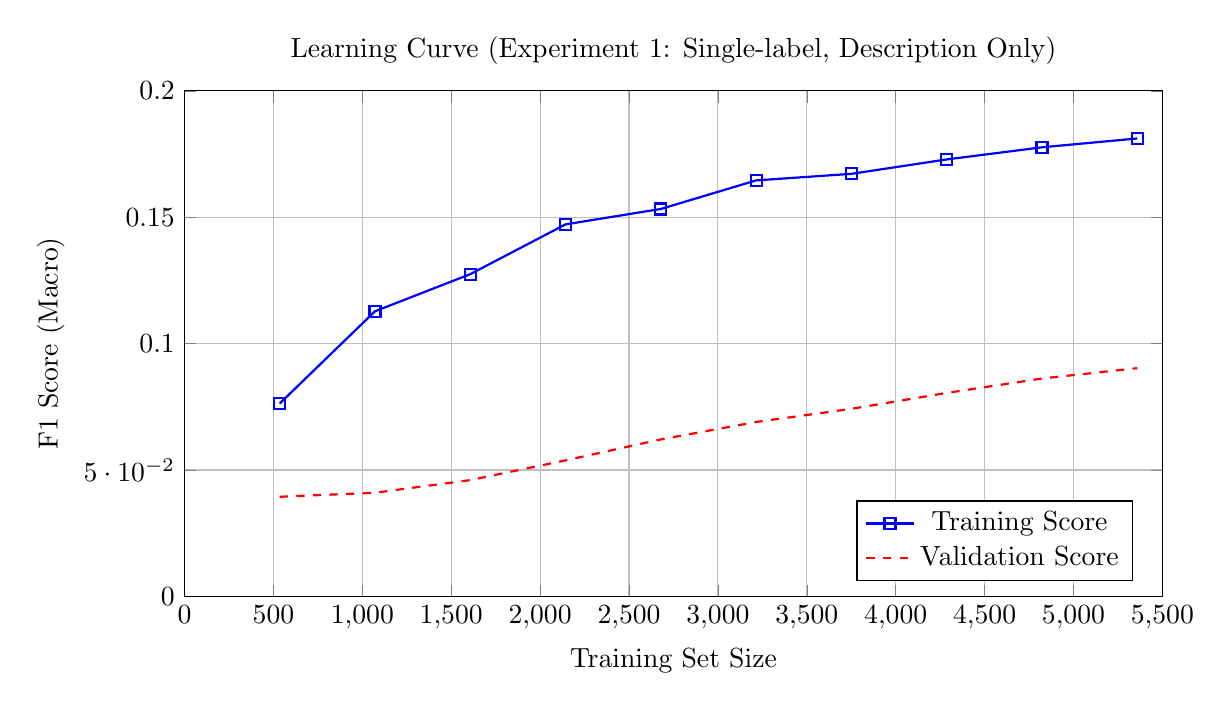
\begin{tikzpicture}
\begin{axis}[
    width=14cm,
    height=8cm,
    xlabel={Training Set Size},
    ylabel={F1 Score (Macro)},
    title={Learning Curve (Experiment 1: Single-label, Description Only)},
    legend pos=south east,
    grid=major,
    xmin=0,
    xmax=5500,
    ymin=0,
    ymax=0.2
]
\addplot[color=blue, thick, mark=square] coordinates {
    (535, 0.0763)
    (1071, 0.1128)
    (1607, 0.1275)
    (2143, 0.1472)
    (2679, 0.1533)
    (3215, 0.1646)
    (3751, 0.1672)
    (4287, 0.1729)
    (4823, 0.1777)
    (5359, 0.1812)
};
\addplot[color=red, thick, mark=circle, dashed] coordinates {
    (535, 0.0394)
    (1071, 0.0410)
    (1607, 0.0460)
    (2143, 0.0538)
    (2679, 0.0621)
    (3215, 0.0690)
    (3751, 0.0742)
    (4287, 0.0805)
    (4823, 0.0862)
    (5359, 0.0903)
};
\legend{Training Score, Validation Score}
\end{axis}
\end{tikzpicture}
\caption{Learning curve showing model performance vs. training set size. The significant gap between training and validation scores indicates overfitting, especially with smaller datasets.}
\label{fig:exp1_learning}
\end{figure}

\subsubsection{Per-Class Performance}

The following analysis shows the F1-score achieved for each genre class. This helps identify which genres are easier or more difficult to predict accurately.

\begin{itemize}
    \item \textbf{Best performing genres}: Romance (F1=0.55), Drama (F1=0.47), Horror (F1=0.46)
    \item \textbf{Moderate performance}: Comedy (F1=0.34), Crime (F1=0.34), Thriller (F1=0.31)
    \item \textbf{Challenging genres}: Action (F1=0.27), Science Fiction (F1=0.27), Adventure (F1=0.22), Fantasy (F1=0.18)
\end{itemize}

The results indicate that Romance, Drama, and Horror genres have more distinctive textual features in movie descriptions, making them easier to classify. Fantasy and Adventure genres show lower performance, possibly due to overlapping themes with other genres.

\begin{figure}[h]
\centering
\begin{tikzpicture}
\begin{axis}[
    xbar,
    xlabel={F1 Score},
    ylabel={Genre},
    width=12cm,
    height=10cm,
    ytick=data,
    xmin=0,
    xmax=0.6,
    title={F1 Score per Genre (Experiment 1: Single-label, Description Only)}
]
\addplot coordinates {
    (0.55,Romance)
    (0.47,Drama)
    (0.46,Horror)
    (0.34,Comedy)
    (0.34,Crime)
    (0.31,Thriller)
    (0.27,Action)
    (0.27,Science Fiction)
    (0.22,Adventure)
    (0.18,Fantasy)
};
\end{axis}
\end{tikzpicture}
\caption{F1-score per genre for single-label classification with description only}
\label{fig:exp1_per_class}
\end{figure}

\subsection{Experiment 2: Single-Label Classification -- Description + Reviews}

\subsubsection{Results}

\begin{itemize}

    \item \textbf{Accuracy}: 60.20\%

    \item \textbf{Macro F1-score}: 0.11

    \item \textbf{Micro F1-score}: 0.60

    \item \textbf{Match Accuracy (any match)}: 62.39\%

\end{itemize}

\subsubsection{Learning Process}

\begin{figure}[h]
\centering
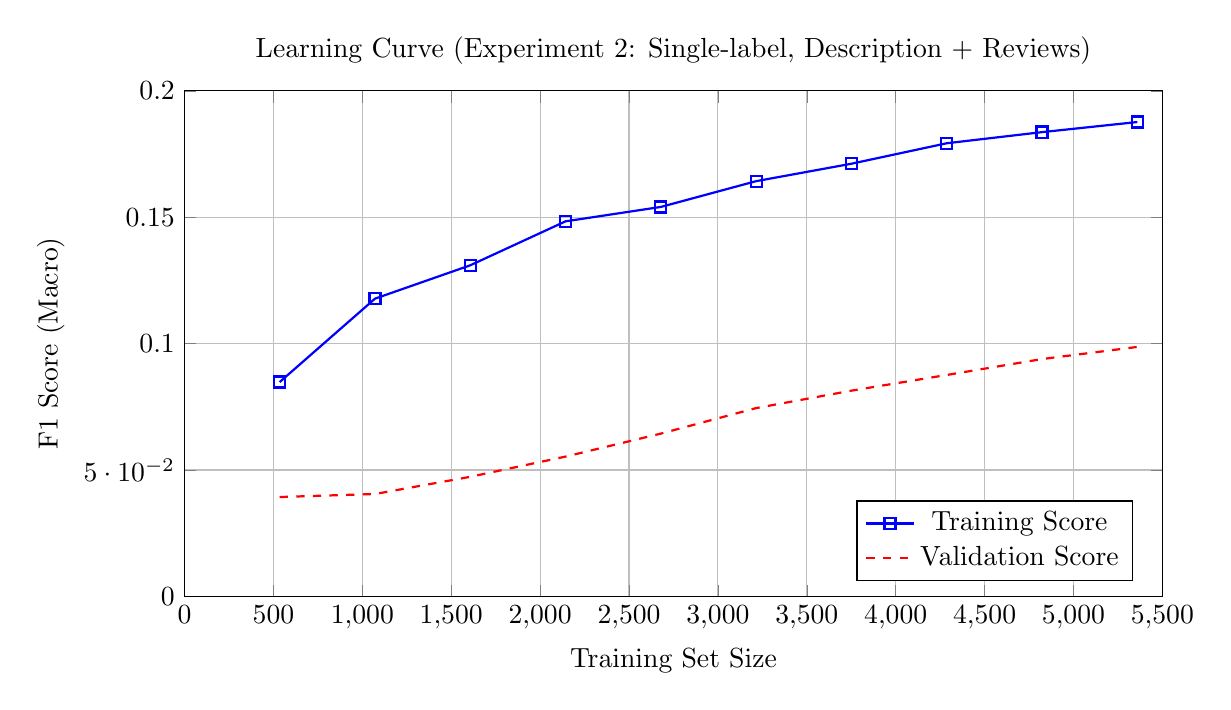
\begin{tikzpicture}
\begin{axis}[
    width=14cm,
    height=8cm,
    xlabel={Training Set Size},
    ylabel={F1 Score (Macro)},
    title={Learning Curve (Experiment 2: Single-label, Description + Reviews)},
    legend pos=south east,
    grid=major,
    xmin=0,
    xmax=5500,
    ymin=0,
    ymax=0.2
]
\addplot[color=blue, thick, mark=square] coordinates {
    (535, 0.0848)
    (1071, 0.1178)
    (1607, 0.1310)
    (2143, 0.1484)
    (2679, 0.1541)
    (3215, 0.1643)
    (3751, 0.1712)
    (4287, 0.1793)
    (4823, 0.1837)
    (5359, 0.1877)
};
\addplot[color=red, thick, mark=circle, dashed] coordinates {
    (535, 0.0393)
    (1071, 0.0405)
    (1607, 0.0473)
    (2143, 0.0553)
    (2679, 0.0644)
    (3215, 0.0745)
    (3751, 0.0814)
    (4287, 0.0876)
    (4823, 0.0939)
    (5359, 0.0987)
};
\legend{Training Score, Validation Score}
\end{axis}
\end{tikzpicture}
\caption{Learning curve for experiment with reviews. The model shows similar learning pattern but slightly better validation scores compared to description-only experiment.}
\label{fig:exp2_learning}
\end{figure}

\subsubsection{Per-Class Performance}

The addition of user reviews provides additional context that helps improve classification for certain genres. The analysis shows:

\begin{itemize}
    \item \textbf{Best performing genres}: Romance (F1=0.55), Drama (F1=0.55), Horror (F1=0.52)
    \item \textbf{Improved with reviews}: Horror shows improvement from 0.46 to 0.52, Crime from 0.34 to 0.33
    \item \textbf{Challenging genres}: Fantasy (F1=0.18) and Adventure (F1=0.21) remain difficult to predict
\end{itemize}

User reviews often contain genre-specific language and emotional expressions that help distinguish genres like Horror (mentions of fear, suspense) and Romance (emotional language, relationship themes).

\begin{figure}[h]
\centering
\begin{tikzpicture}
\begin{axis}[
    xbar,
    xlabel={F1 Score},
    ylabel={Genre},
    width=12cm,
    height=10cm,
    ytick=data,
    xmin=0,
    xmax=0.6,
    title={F1 Score per Genre (Experiment 2: Single-label, Description + Reviews)}
]
\addplot coordinates {
    (0.55,Romance)
    (0.55,Drama)
    (0.52,Horror)
    (0.39,Comedy)
    (0.33,Crime)
    (0.28,Thriller)
    (0.28,Action)
    (0.26,Science Fiction)
    (0.21,Adventure)
    (0.18,Fantasy)
};
\end{axis}
\end{tikzpicture}
\caption{F1-score per genre for single-label classification with description and reviews}
\label{fig:exp2_per_class}
\end{figure}

\textbf{Conclusion}: Adding reviews slightly improves classification quality, especially for Horror and Crime genres.

\subsection{Experiment 3: Multi-Label Classification -- Description Only}

\subsubsection{Results}

\begin{itemize}

    \item \textbf{Hamming Loss}: 0.056

    \item \textbf{Precision (Micro)}: 0.76

    \item \textbf{Recall (Micro)}: 0.09

    \item \textbf{Micro F1-score}: 0.16

    \item \textbf{Precision@k}: 0.42

\end{itemize}

\subsubsection{Learning Process}

\begin{figure}[h]
\centering
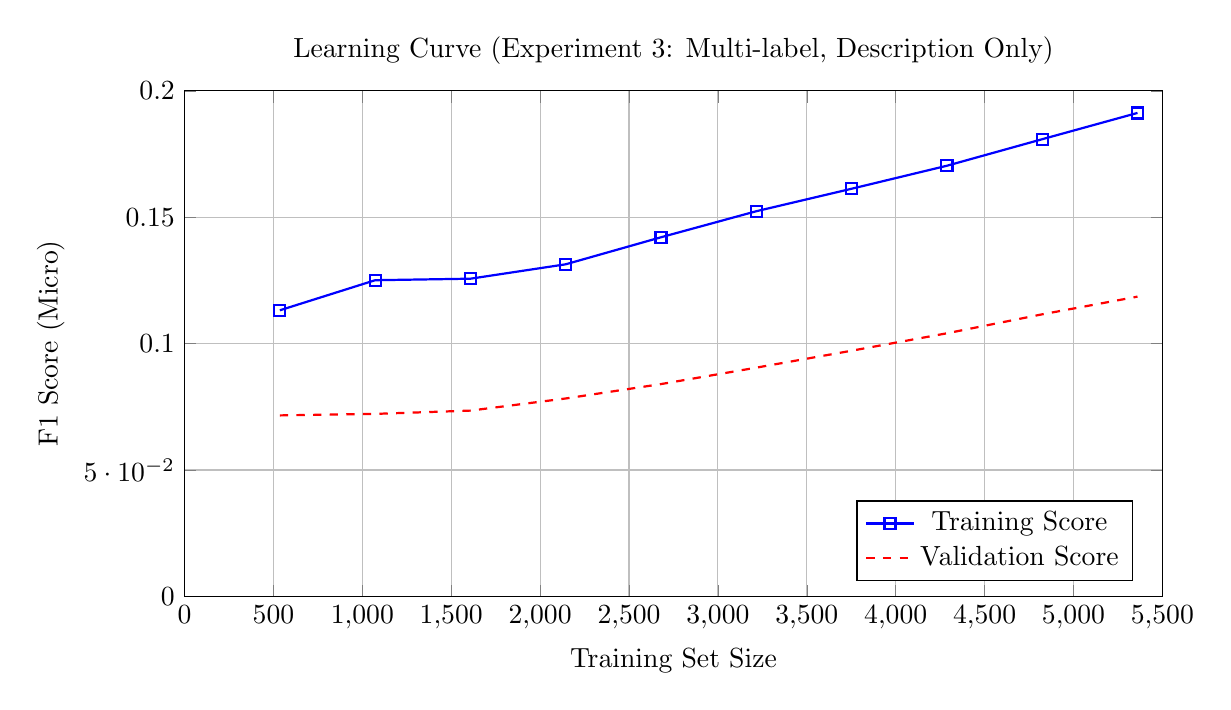
\begin{tikzpicture}
\begin{axis}[
    width=14cm,
    height=8cm,
    xlabel={Training Set Size},
    ylabel={F1 Score (Micro)},
    title={Learning Curve (Experiment 3: Multi-label, Description Only)},
    legend pos=south east,
    grid=major,
    xmin=0,
    xmax=5500,
    ymin=0,
    ymax=0.2
]
\addplot[color=blue, thick, mark=square] coordinates {
    (536, 0.1132)
    (1072, 0.1251)
    (1608, 0.1257)
    (2144, 0.1314)
    (2680, 0.1421)
    (3216, 0.1524)
    (3752, 0.1613)
    (4288, 0.1704)
    (4824, 0.1809)
    (5360, 0.1913)
};
\addplot[color=red, thick, mark=circle, dashed] coordinates {
    (536, 0.0716)
    (1072, 0.0722)
    (1608, 0.0735)
    (2144, 0.0783)
    (2680, 0.0840)
    (3216, 0.0905)
    (3752, 0.0972)
    (4288, 0.1041)
    (4824, 0.1116)
    (5360, 0.1186)
};
\legend{Training Score, Validation Score}
\end{axis}
\end{tikzpicture}
\caption{Learning curve for multi-label classification. The model shows steady improvement with more training data, with validation scores gradually increasing.}
\label{fig:exp3_learning}
\end{figure}

\subsubsection{Per-Genre Performance}

In multi-label classification, each genre is predicted independently, allowing for multiple genres per movie. The per-genre F1-scores show:

\begin{itemize}
    \item \textbf{Best performing genres}: Romance (F1=0.58), Horror (F1=0.56), Crime (F1=0.52), Action (F1=0.50)
    \item \textbf{Moderate performance}: Thriller (F1=0.44), Adventure (F1=0.44), Science Fiction (F1=0.41), Drama (F1=0.39)
    \item \textbf{Challenging genres}: Comedy (F1=0.25), Fantasy (F1=0.25)
\end{itemize}

Multi-label classification shows different performance patterns compared to single-label. Romance and Horror maintain strong performance, while Comedy and Fantasy remain challenging, possibly due to their frequent co-occurrence with other genres.

\begin{figure}[h]
\centering
\begin{tikzpicture}
\begin{axis}[
    xbar,
    xlabel={F1 Score},
    ylabel={Genre},
    width=12cm,
    height=10cm,
    ytick=data,
    xmin=0,
    xmax=0.7,
    title={F1 Score per Genre (Experiment 3: Multi-label, Description Only)}
]
\addplot coordinates {
    (0.58,Romance)
    (0.56,Horror)
    (0.52,Crime)
    (0.50,Action)
    (0.44,Thriller)
    (0.44,Adventure)
    (0.41,Science Fiction)
    (0.39,Drama)
    (0.25,Comedy)
    (0.25,Fantasy)
};
\end{axis}
\end{tikzpicture}
\caption{F1-score per genre for multi-label classification with description only}
\label{fig:exp3_per_class}
\end{figure}

\subsection{Experiment 4: Multi-Label Classification -- Description + Reviews}

\subsubsection{Results}

\begin{itemize}

    \item \textbf{Hamming Loss}: 0.106

    \item \textbf{Precision (Micro)}: 0.80

    \item \textbf{Recall (Micro)}: 0.27

    \item \textbf{Micro F1-score}: 0.41

    \item \textbf{Precision@k}: 0.62

\end{itemize}

\subsubsection{Learning Process}

\begin{figure}[h]
\centering
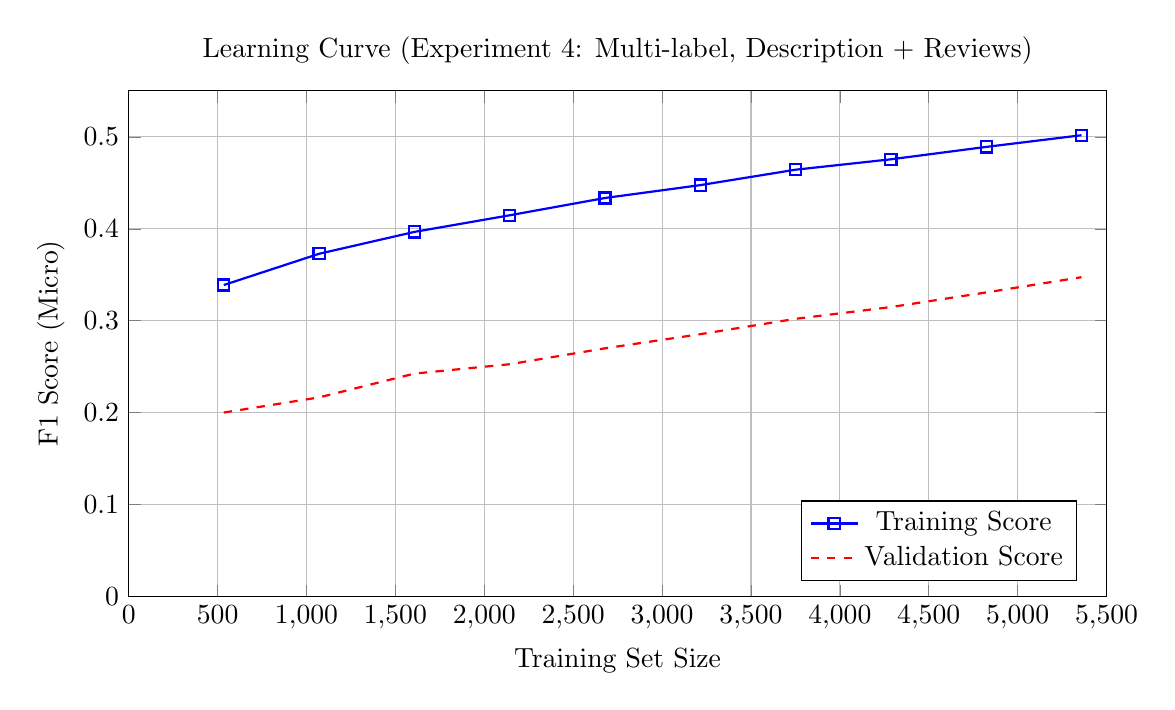
\begin{tikzpicture}
\begin{axis}[
    width=14cm,
    height=8cm,
    xlabel={Training Set Size},
    ylabel={F1 Score (Micro)},
    title={Learning Curve (Experiment 4: Multi-label, Description + Reviews)},
    legend pos=south east,
    grid=major,
    xmin=0,
    xmax=5500,
    ymin=0,
    ymax=0.55
]
\addplot[color=blue, thick, mark=square] coordinates {
    (535, 0.3388)
    (1071, 0.3728)
    (1607, 0.3966)
    (2143, 0.4147)
    (2679, 0.4335)
    (3215, 0.4475)
    (3751, 0.4643)
    (4287, 0.4756)
    (4823, 0.4891)
    (5359, 0.5018)
};
\addplot[color=red, thick, mark=circle, dashed] coordinates {
    (535, 0.2000)
    (1071, 0.2165)
    (1607, 0.2424)
    (2143, 0.2526)
    (2679, 0.2699)
    (3215, 0.2853)
    (3751, 0.3020)
    (4287, 0.3148)
    (4823, 0.3307)
    (5359, 0.3473)
};
\legend{Training Score, Validation Score}
\end{axis}
\end{tikzpicture}
\caption{Learning curve for multi-label classification with reviews. The model achieves significantly better performance compared to description-only version, with validation scores reaching 0.35.}
\label{fig:exp4_learning}
\end{figure}

\subsubsection{Per-Genre Performance}

The combination of descriptions and reviews significantly improves multi-label classification performance across most genres:

\begin{itemize}
    \item \textbf{Best performing genres}: Horror (F1=0.67), Romance (F1=0.58), Action (F1=0.54), Thriller (F1=0.51)
    \item \textbf{Notable improvements}: Horror improves from 0.56 to 0.67, Action from 0.50 to 0.54
    \item \textbf{Moderate performance}: Drama (F1=0.48), Crime (F1=0.47), Science Fiction (F1=0.43), Adventure (F1=0.39)
    \item \textbf{Challenging genres}: Comedy (F1=0.28), Fantasy (F1=0.25) - still difficult but show slight improvement
\end{itemize}

User reviews provide valuable genre-specific signals, especially for Horror (fear, suspense, scares) and Action (excitement, intensity). The reviews help distinguish genres that might be ambiguous from descriptions alone.

\begin{figure}[h]
\centering
\begin{tikzpicture}
\begin{axis}[
    xbar,
    xlabel={F1 Score},
    ylabel={Genre},
    width=12cm,
    height=10cm,
    ytick=data,
    xmin=0,
    xmax=0.7,
    title={F1 Score per Genre (Experiment 4: Multi-label, Description + Reviews)}
]
\addplot coordinates {
    (0.67,Horror)
    (0.58,Romance)
    (0.54,Action)
    (0.51,Thriller)
    (0.48,Drama)
    (0.47,Crime)
    (0.43,Science Fiction)
    (0.39,Adventure)
    (0.28,Comedy)
    (0.25,Fantasy)
};
\end{axis}
\end{tikzpicture}
\caption{F1-score per genre for multi-label classification with description and reviews}
\label{fig:exp4_per_class}
\end{figure}

\subsection{Experiment 5: Transformer Model (BERT) -- Description + Reviews}

\subsubsection{Results}

\begin{itemize}

    \item \textbf{Hamming Loss}: 0.110

    \item \textbf{Macro F1-score}: 0.63

    \item \textbf{Micro F1-score}: 0.64

\end{itemize}

\subsubsection{Training Process}

The following figures show the training process for the BERT model, demonstrating how the model learned over epochs.

\begin{figure}[h]
\centering
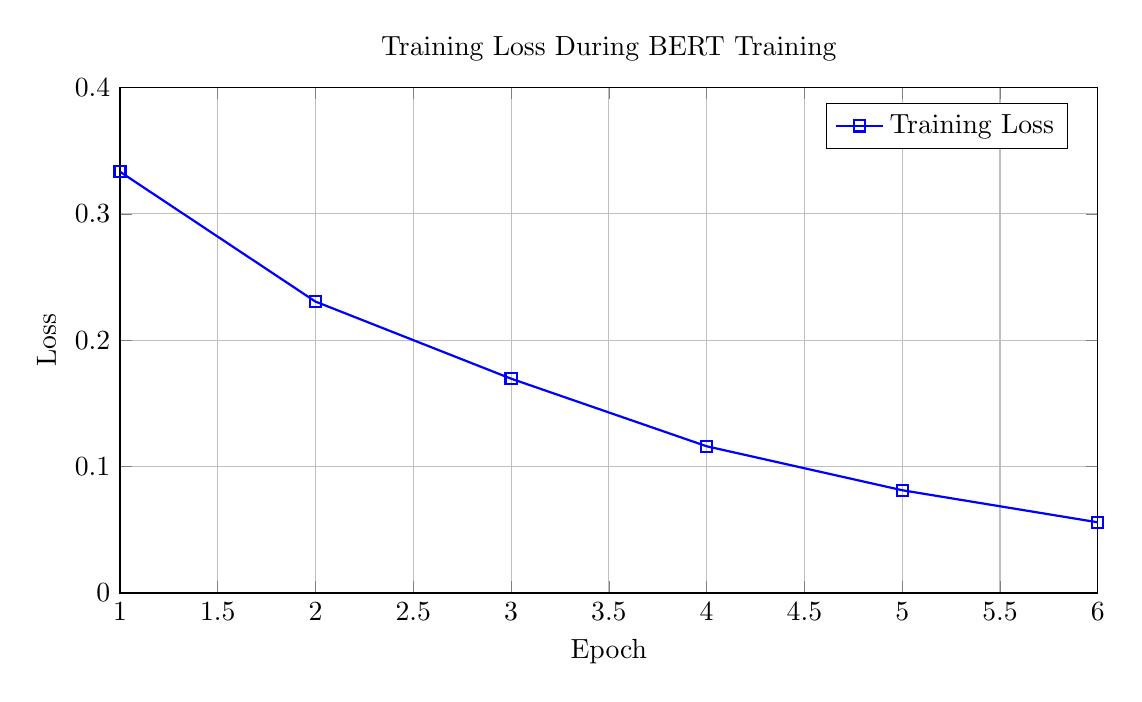
\begin{tikzpicture}
\begin{axis}[
    width=14cm,
    height=8cm,
    xlabel={Epoch},
    ylabel={Loss},
    title={Training Loss During BERT Training},
    legend pos=north east,
    grid=major,
    xmin=1,
    xmax=6,
    ymin=0,
    ymax=0.4
]
\addplot[color=blue, thick, mark=square] coordinates {
    (1, 0.3334)
    (2, 0.2306)
    (3, 0.1696)
    (4, 0.1161)
    (5, 0.0813)
    (6, 0.0559)
};
\legend{Training Loss}
\end{axis}
\end{tikzpicture}
\caption{Training loss decreases over epochs, showing model convergence. Early stopping was triggered at epoch 6.}
\label{fig:training_loss}
\end{figure}

\begin{figure}[h]
\centering
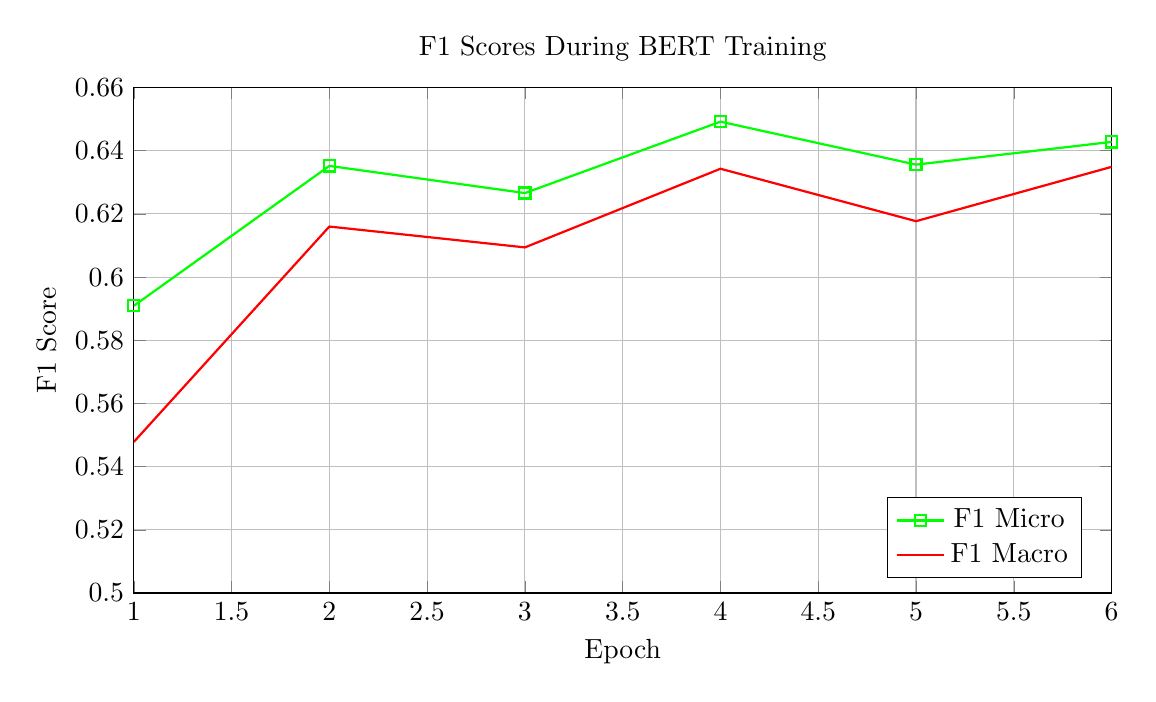
\begin{tikzpicture}
\begin{axis}[
    width=14cm,
    height=8cm,
    xlabel={Epoch},
    ylabel={F1 Score},
    title={F1 Scores During BERT Training},
    legend pos=south east,
    grid=major,
    xmin=1,
    xmax=6,
    ymin=0.5,
    ymax=0.66
]
\addplot[color=green, thick, mark=square] coordinates {
    (1, 0.5909)
    (2, 0.6352)
    (3, 0.6266)
    (4, 0.6492)
    (5, 0.6356)
    (6, 0.6428)
};
\addplot[color=red, thick, mark=circle] coordinates {
    (1, 0.5478)
    (2, 0.6160)
    (3, 0.6094)
    (4, 0.6343)
    (5, 0.6177)
    (6, 0.6349)
};
\legend{F1 Micro, F1 Macro}
\end{axis}
\end{tikzpicture}
\caption{F1 Micro and F1 Macro scores improve over training epochs. The model achieves best performance at epoch 4, after which early stopping prevents overfitting.}
\label{fig:training_f1}
\end{figure}

\begin{figure}[h]
\centering
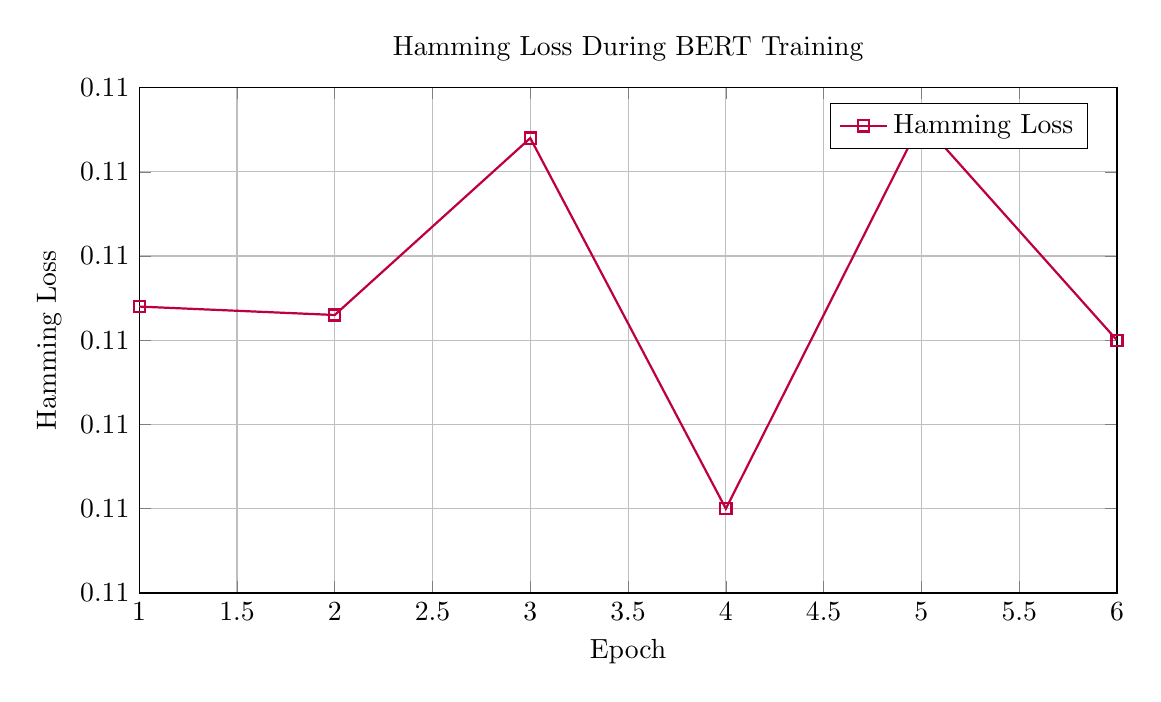
\begin{tikzpicture}
\begin{axis}[
    width=14cm,
    height=8cm,
    xlabel={Epoch},
    ylabel={Hamming Loss},
    title={Hamming Loss During BERT Training},
    legend pos=north east,
    grid=major,
    xmin=1,
    xmax=6,
    ymin=0.107,
    ymax=0.113
]
\addplot[color=purple, thick, mark=square] coordinates {
    (1, 0.1104)
    (2, 0.1103)
    (3, 0.1124)
    (4, 0.1080)
    (5, 0.1126)
    (6, 0.1100)
};
\legend{Hamming Loss}
\end{axis}
\end{tikzpicture}
\caption{Hamming Loss remains relatively stable during training, with best performance at epoch 4 (0.1080). Lower values indicate better multi-label classification performance.}
\label{fig:training_hamming}
\end{figure}

\begin{figure}[h]
\centering
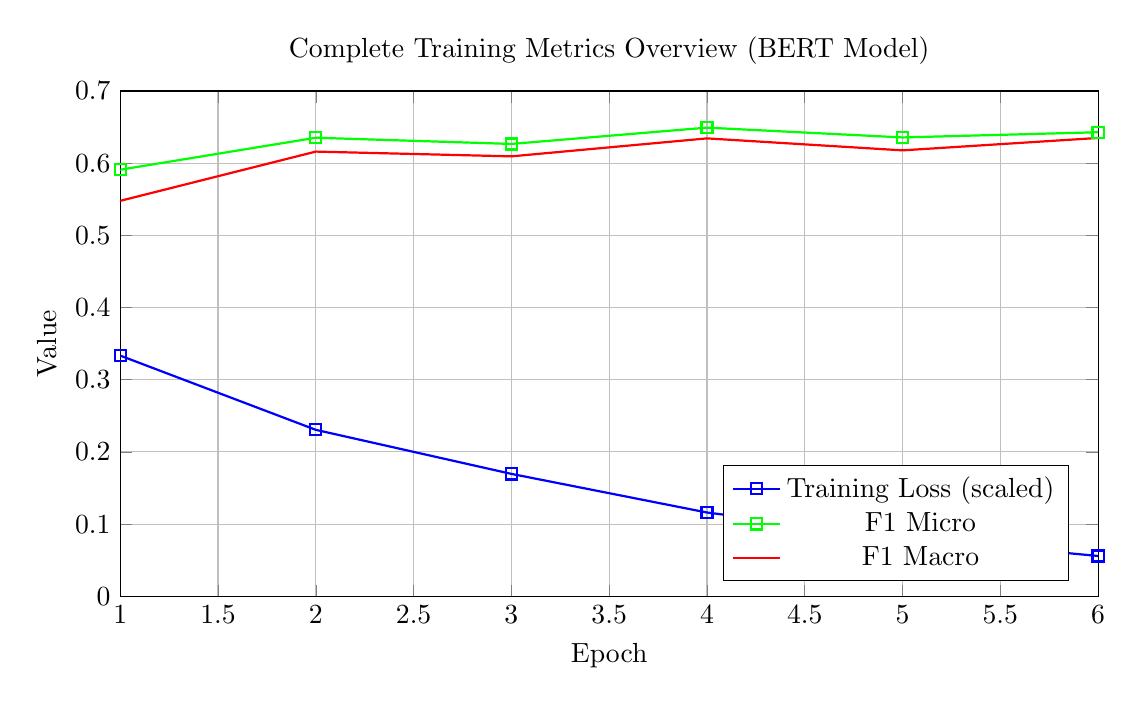
\begin{tikzpicture}
\begin{axis}[
    width=14cm,
    height=8cm,
    xlabel={Epoch},
    ylabel={Value},
    title={Complete Training Metrics Overview (BERT Model)},
    legend pos=south east,
    grid=major,
    xmin=1,
    xmax=6,
    ymin=0,
    ymax=0.7,
    scaled y ticks=false
]
\addplot[color=blue, thick, mark=square] coordinates {
    (1, 0.3334)
    (2, 0.2306)
    (3, 0.1696)
    (4, 0.1161)
    (5, 0.0813)
    (6, 0.0559)
};
\addplot[color=green, thick, mark=square] coordinates {
    (1, 0.5909)
    (2, 0.6352)
    (3, 0.6266)
    (4, 0.6492)
    (5, 0.6356)
    (6, 0.6428)
};
\addplot[color=red, thick, mark=circle] coordinates {
    (1, 0.5478)
    (2, 0.6160)
    (3, 0.6094)
    (4, 0.6343)
    (5, 0.6177)
    (6, 0.6349)
};
\legend{Training Loss (scaled), F1 Micro, F1 Macro}
\end{axis}
\end{tikzpicture}
\caption{Combined view of training metrics showing loss decreasing while F1 scores increase, indicating successful learning. Best model checkpoint was saved at epoch 4.}
\label{fig:training_overview}
\end{figure}

\section{Analysis and Conclusions}

\subsection{Key Observations}

\begin{itemize}

    \item User reviews consistently improve performance

    \item Multi-label classification better reflects real-world data

    \item BERT significantly outperforms classical ML methods

    \item Fantasy and Comedy remain the hardest genres to predict

\end{itemize}

\subsection{Comparison of Experiments}

\begin{table}[h]

\centering

\begin{tabular}{lccccc}

\toprule

\textbf{Metric} & \textbf{Exp1} & \textbf{Exp2} & \textbf{Exp3} & \textbf{Exp4} & \textbf{Exp5} \\

\midrule

Accuracy / Exact Match & 58.51\% & 60.20\% & -- & -- & -- \\

F1 Micro               & 0.59    & 0.60    & 0.16    & 0.41    & 0.64 \\

F1 Macro               & 0.11    & 0.11    & --      & --      & 0.63 \\

Hamming Loss           & --      & --      & 0.056   & 0.106   & 0.110 \\

\bottomrule

\end{tabular}

\caption{Comparison of experimental results (transposed layout)}

\label{tab:results}

\end{table}

\begin{figure}[h]
\centering
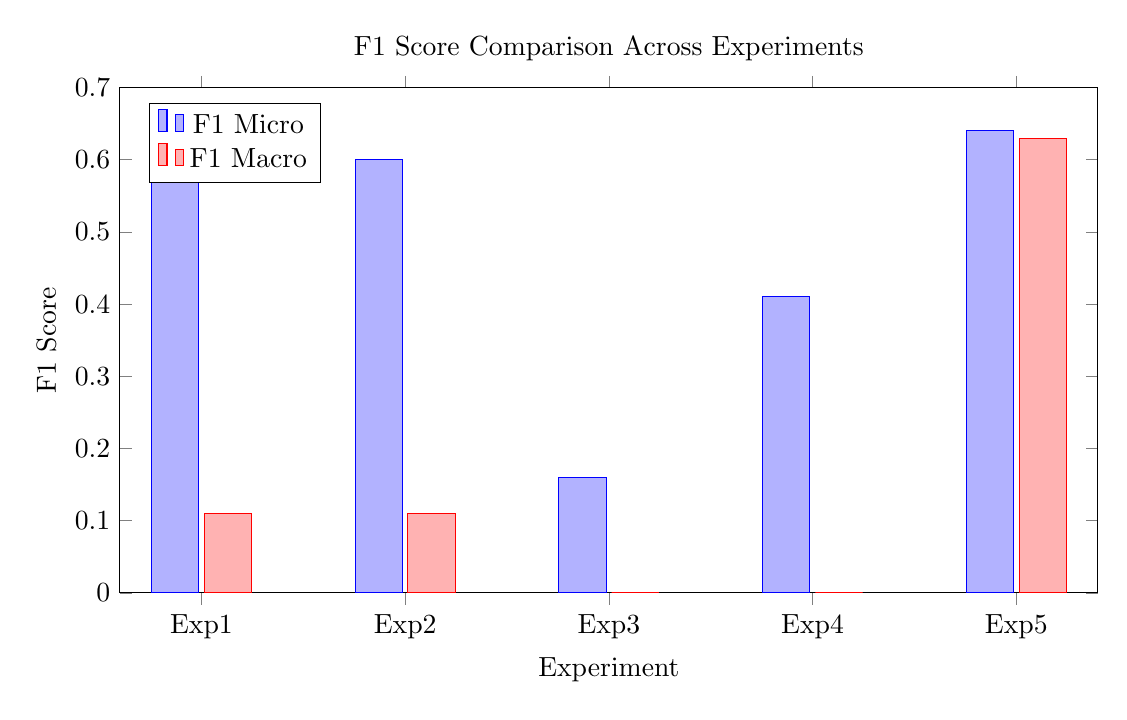
\begin{tikzpicture}
\begin{axis}[
    ybar,
    bar width=0.6cm,
    width=14cm,
    height=8cm,
    ylabel={F1 Score},
    xlabel={Experiment},
    symbolic x coords={Exp1,Exp2,Exp3,Exp4,Exp5},
    xtick=data,
    ymin=0,
    ymax=0.7,
    legend pos=north west,
    title={F1 Score Comparison Across Experiments}
]
\addplot coordinates {(Exp1,0.59) (Exp2,0.60) (Exp3,0.16) (Exp4,0.41) (Exp5,0.64)};
\addplot coordinates {(Exp1,0.11) (Exp2,0.11) (Exp3,0.00) (Exp4,0.00) (Exp5,0.63)};
\legend{F1 Micro, F1 Macro}
\end{axis}
\end{tikzpicture}
\caption{Comparison of F1 Micro and F1 Macro scores across all experiments}
\label{fig:f1_comparison}
\end{figure}

\begin{figure}[h]
\centering
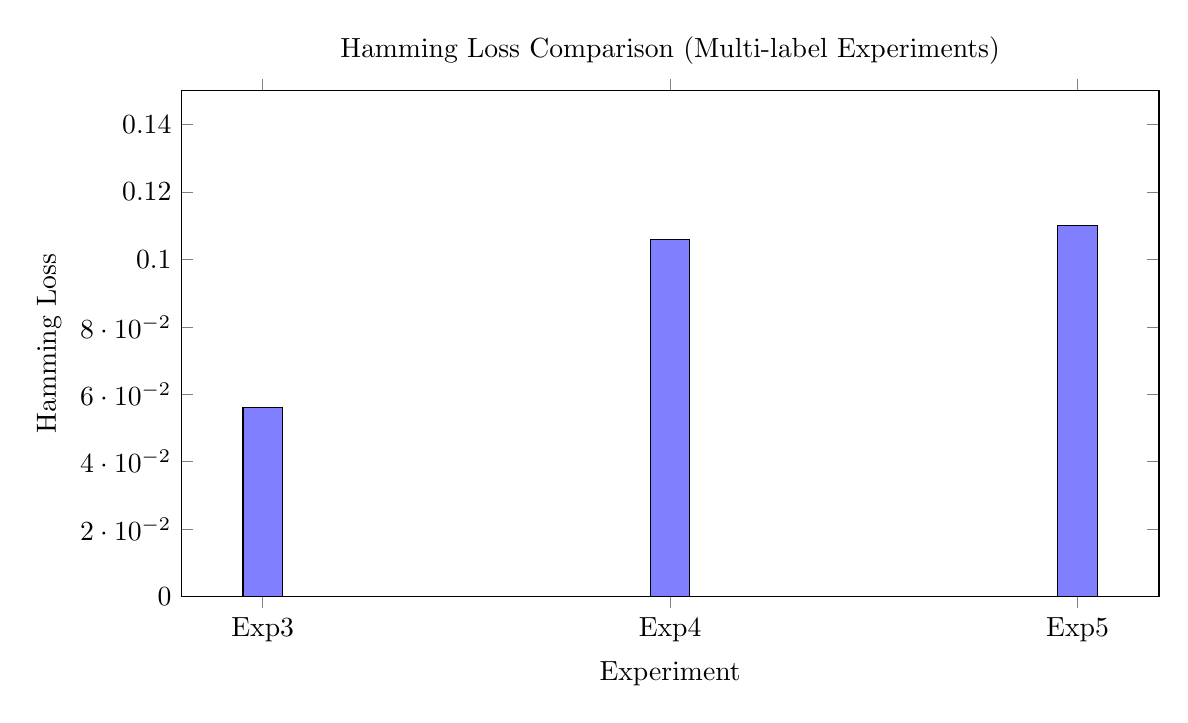
\begin{tikzpicture}
\begin{axis}[
    ybar,
    bar width=0.5cm,
    width=14cm,
    height=8cm,
    ylabel={Hamming Loss},
    xlabel={Experiment},
    symbolic x coords={Exp3,Exp4,Exp5},
    xtick=data,
    ymin=0,
    ymax=0.15,
    title={Hamming Loss Comparison (Multi-label Experiments)},
    bar shift=0pt
]
\addplot[fill=blue!50] coordinates {(Exp3,0.056) (Exp4,0.106) (Exp5,0.110)};
\end{axis}
\end{tikzpicture}
\caption{Hamming Loss comparison for multi-label classification experiments (lower is better)}
\label{fig:hamming_loss}
\end{figure}

\begin{figure}[h]
\centering
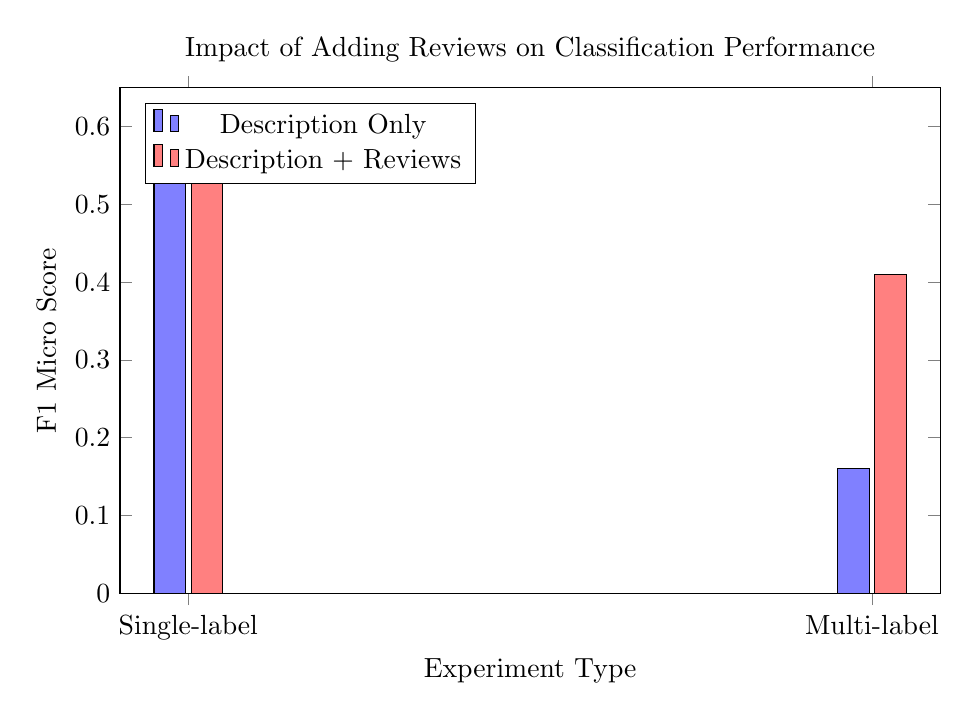
\begin{tikzpicture}
\begin{axis}[
    ybar,
    bar width=0.4cm,
    width=12cm,
    height=8cm,
    ylabel={F1 Micro Score},
    xlabel={Experiment Type},
    symbolic x coords={Single-label,Multi-label},
    xtick=data,
    ymin=0,
    ymax=0.65,
    legend pos=north west,
    title={Impact of Adding Reviews on Classification Performance}
]
\addplot[fill=blue!50] coordinates {(Single-label,0.59) (Multi-label,0.16)};
\addplot[fill=red!50] coordinates {(Single-label,0.60) (Multi-label,0.41)};
\legend{Description Only, Description + Reviews}
\end{axis}
\end{tikzpicture}
\caption{Comparison showing improvement when reviews are added to descriptions}
\label{fig:review_impact}
\end{figure}

\end{document}

